\documentclass[crop,tikz]{standalone} 
\usepackage{tikz, amsmath, amssymb, graphicx} 

\DeclareMathAlphabet\mathbfcal{OMS}{cmsy}{b}{n}

\newcommand{\Mt}{\mathbfcal{M}}
\newcommand{\Yt}{\mathbfcal{Y}}
\newcommand{\Ft}{\mathbfcal{F}}

\usetikzlibrary{positioning, shapes.geometric} 

\begin{document}  

\tikzset{fontscale/.style = {font=\relsize{#1}}
    }
 
\begin{tikzpicture} 

 
\node[inner sep=0pt] at (0, 0) {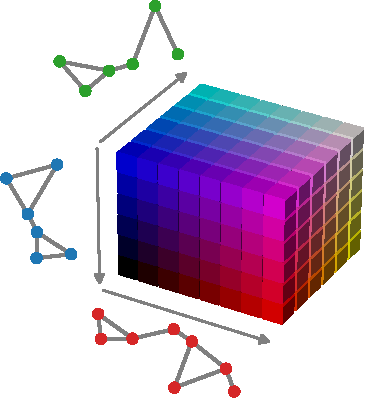
\includegraphics[width=.22\textwidth]{coloured_tensor.pdf}};

\node[inner sep=0pt, scale=0.6] at (-1.5, -0.2) {$\mathcal{G}_1$};
\node[inner sep=0pt, scale=0.6] at (-0.5, -1.4) {$\mathcal{G}_2$};
\node[inner sep=0pt, scale=0.6] at (-0.7, 1.3) {$\mathcal{G}_3$};

\end{tikzpicture}
\end{document} 
